%% 
%% Copyright 2019-2020 Elsevier Ltd
%% 
%% This file is part of the 'CAS Bundle'.
%% --------------------------------------
%% 
%% It may be distributed under the conditions of the LaTeX Project Public
%% License, either version 1.2 of this license or (at your option) any
%% later version.  The latest version of this license is in
%%    http://www.latex-project.org/lppl.txt
%% and version 1.2 or later is part of all distributions of LaTeX
%% version 1999/12/01 or later.
%% 
%% The list of all files belonging to the 'CAS Bundle' is
%% given in the file `manifest.txt'.
%% 
%% Template article for cas-sc documentclass for 
%% double column output.

% \documentclass[a4paper,fleqn,longmktitle]{cas-sc}
\documentclass[a4paper]{cas-sc}
% \documentclass{article}
% \usepackage[numbers]{natbib}
\usepackage[authoryear]{natbib}
\UseRawInputEncoding
% \usepackage[authoryear,longnamesfirst]{natbib}
% \renewcommand {\thetable} {\arabic{table}}

% \renewcommand {\thefigure} {\arabic{figure}}
\usepackage{chngcntr}%需要调用这个宏包
\counterwithout{figure}{section}%
\usepackage{threeparttable}
% \usepackage[section]{placeins}
\usepackage{afterpage}
% \usepackage[disable]{endfloat}
\usepackage{amsmath}
\usepackage{ntheorem}
\usepackage{subcaption}
\usepackage{mwe}
\newtheorem{theorem}{Theorem}
\newtheorem{lemma}[theorem]{Lemma}
\newtheorem*{proof}{Proof}
\newtheorem{remark}[theorem]{Remark}
\newtheorem{defi}[theorem]{Definition}
\newtheorem{property}[theorem]{Property}
\newtheorem{corollary}[theorem]{Corollary}
% \usepackage[section,above]{placeins}

%%%Author definitions
\def\tsc#1{\csdef{#1}{\textsc{\lowercase{#1}}\xspace}}
\tsc{WGM}
\tsc{QE}
\tsc{EP}
\tsc{PMS}
\tsc{BEC}
\tsc{DE}
%%%


\begin{document}
\let\WriteBookmarks\relax
\def\floatpagepagefraction{1}
\def\textpagefraction{.001}


% Short author
\shortauthors{Tiancheng Ruan et~al.}
\shorttitle{}

% Main title of the paper
\title [mode = title]{Modeling and stability analysis of the general Cooperative Adaptive Cruise Control platoon considering a rate-free time-varying communication delay and uncertainties}
% Title footnote mark
% eg: \tnotemark[1]
% \tnotemark[1,2]

% Title footnote 1.
% eg: \tnotetext[1]{Title footnote text}
% \tnotetext[<tnote number>]{<tnote text>} 
% \tnotetext[1]{This document is the results of the research
%    project funded by the National Science Foundation.}

% \tnotetext[2]{The second title footnote which is a longer text matter
%    to fill through the whole text width and overflow into
%    another line in the footnotes area of the first page.}


% First author
%
% Options: Use if required
% eg: \author[1,3]{Author Name}[type=editor,
%       style=chinese,
%       auid=000,
%       bioid=1,
%       prefix=Sir,
%       orcid=0000-0000-0000-0000,
%       twitter=<twitter id>,
%       linkedin=<linkedin id>,
%       gplus=<gplus id>]
\author[1,2,3]{Tiancheng Ruan}[style=chinese]
\ead{ruantiancheng@seu.edu.cn}
\credit{Conceptualization of this study, Methodology, Writing - Original draft preparation, Resources, Software}

\author[1,2,3]{Yu Chen}[style=chinese]
\ead{230228902@seu.edu.cn}
\credit{Software, Validation, Visualization}


\author[1,2,3]{Hao Wang}[style=chinese]
% Corresponding author indication
\cormark[1]

% % Footnote of the first author
% \fnmark[1]

% Email id of the first author
\ead{haowang@seu.edu.cn}

% % URL of the first author
% \ead[url]{www.cvr.cc, cvr@sayahna.org}

%  Credit authorship
\credit{ Formal analysis, Funding acquisition, Supervision,Writing - review \& editing}

% Address/affiliation
\affiliation[1]{organization={Jiangsu Key Laboratory of Urban ITS, Southeast University},
  addressline={2 Si Pai Lou},
  city={Nanjing},
  postcode={210096},
  % state={},
  country={P.R. China}}

\affiliation[2]{organization={Jiangsu Province Collaborative Innovation Center of Modern Urban Traffic Technologies},
  addressline={2 Si Pai Lou},
  city={Nanjing},
  postcode={210096},
  % state={},
  country={P.R. China}}
\affiliation[3]{organization={School of Transportation, Southeast University},
  addressline={2 Si Pai Lou},
  city={Nanjing},
  postcode={210096},
  % state={},
  country={P.R. China}}
% Second author

\author[4]{Xiaopeng Li}[style=chinese]
% \fnmark[2]
\ead{xli2485@wisc.edu}
% \ead[URL]{www.sayahna.org}
\credit{Writing - Original draft preparation,Writing - review \& editing, Supervision}

\affiliation[4]{organization={Department of Civil \& Environmental Engineering, University of Wisconsin-Madison},
  addressline={1415 Engineering Drive},
  city={Madison},
  % citysep={}, % Uncomment if no comma needed between city and postcode
  postcode={53706},
  % state={},
  country={USA}}

% Third author
\author[1,2,3]{Jian Wang}[style=chinese]
% \fnmark[2]
\ead{jianw@seu.edu.cn}
% \ead[URL]{www.sayahna.org}
\credit{Data curation, Formal analysis, Investigation, Supervision}

\author[1,2,3]{Yi Liu}[style=chinese]
\ead{dlmu_liuyi@163.com}
\credit{Formal analysis, Software}

% Corresponding author text
\cortext[cor1]{Corresponding author}

% Footnote text
% \fntext[fn1]{This is the first author footnote. but is common to third
%   author as well.}
% \fntext[fn2]{Another author footnote, this is a very long footnote and
%   it should be a really long footnote. But this footnote is not yet
%   sufficiently long enough to make two lines of footnote text.}

% For a title note without a number/mark
% \nonumnote{This note has no numbers. In this work we demonstrate $a_b$
%   the formation Y\_1 of a new type of polariton on the interface
%   between a cuprous oxide slab and a polystyrene micro-sphere placed
%   on the slab.
%   }





% Here goes the abstract
\begin{abstract}
  In recent years, Cooperative Adaptive Cruise Controls (CACCs) have gradually become a promising solution to problems such as traffic congestion and pollutant emissions, with significant research supporting their effectiveness. This is all based on meeting the fundamental control objective of stability. However, widely used feedback control cannot guarantee absolute stability due to the inevitable presence of communication delays. As a result, numerous research efforts have been conducted to derive stability conditions that consider communication delays. However, the time-varying and rate-free attributes of communication delay make deriving stability conditions highly challenging. Therefore, this paper establishes a general representation for a CACC platoon considering a rate-free communication delay. Building upon this representation, a novel stability condition for a CACC platoon considering a rate-free communication delay is derived using the Lyapunov-Krasovskii Stability Theorem and Schur complement to address the rate-free attribute. Furthermore, another robust stability condition is deduced, considering the presence of measurement uncertainties. Additionally, extensive numerical analyses are conducted to investigate the impact of a rate-free communication delay and measurement uncertainties on tracking performance, transient response, and safety conditions. The results indicate that all CACCs can effectively track errors and achieve equilibrium if the stability condition is fulfilled. Furthermore, realistic scenarios with a rate-free communication delay and measurement uncertainties exhibit poorer tracking performance, transient response, and safety conditions than ideal scenarios featuring constant communication delay. Also, CACCs with access to more distant and diverse information demonstrate superior transient response and safety conditions.
\end{abstract}

% Use if graphical abstract is present
% \begin{graphicalabstract}
% \includegraphics{figs/grabs.pdf}
% \end{graphicalabstract}

% Research highlights
\begin{highlights}
  \item A general supermatrix modeling approach is proposed for the CACC platoon, which takes into account a rate-free communication delay.
  \item Two novel stability conditions for the CACC platoon considering a rate-free communication delay, with or without system uncertainties, are derived based on the Lyapunov-Krasovskii Stability Theorem and Schur complement.
  \item A comprehensive performance evaluation analysis is conducted to comprehensively assess the impact of a rate-free communication delay and uncertainties on tracking performance, transient response, and safety conditions.
\end{highlights}

% Keywords
% Each keyword is seperated by \sep
\begin{keywords}
  Cooperative Adaptive Cruise Control (CACC); CACC platoon; State-space modeling; Stability analysis; rate-free communication delay; system uncertainty.
\end{keywords}


\maketitle

\section{Introduction}
\label{Section 1}

In the last decade, the development of automation technology has led to the emergence of Automated Vehicles (AVs), which have become a popular and widely studied topic in both academia and industry. AVs benefit from automatic control, allowing them to perceive changes in the surrounding environment through on-board sensors and make decisions accordingly \citep{SHLADOVER1978}. As they are not subject to the heterogeneity of human factors that can lead to uncertainty \citep{Arem2016a,Yu2021a,vanLint2016}, AVs are considered a promising solution to address current issues such as traffic congestion \citep{Zhao2020,Wang2019b}, traffic accidents \citep{Ruan2022,Wang2018g}, and pollutant emissions \citep{Silgu2020,Wang2020f,wang2022worst}.

One of the most widely researched examples of AVs is the Adaptive Cruise Control (ACC) strategy. ACCs employ various on-board sensors to detect the real-time position and speed of the preceding vehicle. Based on the detected dynamic information, ACCs can achieve specific control objectives, such as maintaining a desired time headway or distance with the predecessor \citep{fancher1997tests, marsden2001towards}. Although research has demonstrated the superiority of ACCs over Human-Driven Vehicles in terms of safety \citep{vahidi2003research, mahdinia2020safety} and eco-driving \citep{wang2014potential, li2019ecological}, their capacity gains are uncertain \citep{vander2002effects, shang2021impacts}. This is because the actual response time of the vehicle controller, which includes measurement delay, parasitic delay, engine actuator lag, and other factors, deteriorates the mobility of ACCs, despite their theoretical ability to respond within a very short time frame \citep{xiao2008stability}. Recent research estimates the equivalent response time based on field experiment data to be in the range of $0.8s-1.2s$, which is similar to the general assumption of human drivers \citep{makridis2019response}.


Recent advancements in Cellular Vehicle-to-Everything (C-V2X) and wireless communication technology have made Cooperative Adaptive Cruise Control (CACC) a promising solution \citep{hua2020influence,yu2022safety}. CACCs are capable of utilizing Vehicle-to-Infrastructure (V2I) and Vehicle-to-Vehicle (V2V) communication to share information among the CACC platoon \citep{Wang2022,Qin2021a}, enabling them to make better decisions compared to ACCs, which rely solely on on-board sensors. Additionally, using Basic Safety Messages from multiple vehicles allows the CACC to reduce inter-vehicle spacing without compromising safety. By ensuring safety with shorter inter-vehicle distances, CACCs have the potential to nearly double the road capacity compared to ACCs with 100\% market penetration \citep{Xing2020,ruan2021stability}. Furthermore, several studies have investigated the benefits of CACCs in terms of capacity \citep{Gong2018a,yu2022stability}, stability \citep{Zhou2019c,Talebpour2017a}, and pollutant emissions \citep{Wang2022,schmied2015nonlinear}.




Although CACCs have demonstrated advantages in various aspects, ensuring their stability is a fundamental requirement for realizing these benefits \citep{orosz2016connected}. In particular, the transient response of CACCs to disturbances should diminish over time \citep{jiang2018experimental}. However, the presence of communication delay means that stability cannot be absolutely guaranteed with the widely used feedback control method \citep{amirkhani2022consensus,bao2022recent}. The timing of a system's response can be affected by communication delays, which may result in phase shifts. Implementing feedback control to stabilize a system with time delays may lead to issues in addressing this challenge. The stability domain could become smaller, and the possibility of overcompensation could increase. Overcompensation occurs when a system's corrective actions are too strong, leading to unwanted oscillations or instability instead of achieving the desired stability. As a result, extensive research has been dedicated to deriving stability conditions for CACCs that account for delays \citep{herman1959traffic, zhang1997stability, li2010lyapunov, li2013stability, kamath2015car, sun_stability_2018}.

Current research utilizes various methods that can be broadly categorized into two main groups: frequency domain-based methods and time domain-based methods. In the early stages of research, the frequency domain-based method was commonly used to derive stability conditions, as demonstrated by Chandler et al. \citep{chandler1958traffic} and Gazis et al. \citep{gazis1959car}. This method involved fitting the vehicle dynamics into a simple linear time-delay model and using Laplace transform-based techniques to obtain the corresponding characteristic equations. Subsequently, stability conditions were derived through both numerical and theoretical methods \citep{herman1959traffic,zhang1997stability}. Hajdu et al. represented vehicle dynamics as a transfer function that includes uncertainty and time delay, and obtained stability conditions numerically using Nyquist diagrams and Bode plots \citep{hajdu2016robust}. In a similar vein, Molnar et al. modeled vehicle motion as a double integrator with saturation and integrated delay, and derived a transfer function for the vehicle platoon that accounts for delay. They then fitted a delay-free transfer function with similar dynamic performance as the delay-dependent one, and derived corresponding stability conditions based on the poles of the transfer function \citep{molnar2022virtual}. In frequency domain-based methods, communication delay is represented by the expression $e^{-j\omega\tau}$, where $\omega$ signifies the angular frequency, and $\tau$ denotes the communication delay. This delay term, which implies a frequency-dependent phase shift, results in continuous phase alterations throughout the entire frequency spectrum, consequently causing high dimensionality. This increased dimensionality presents a significant obstacle when attempting to analytically derive stability conditions for frequency domain-based methods. The high dimensionality is a result of the intricacies associated with functional differential equations. These equations involve functions that depend on both the current and past values of the variables, in contrast to ordinary differential equations, which only take into account the current values. The consideration of past values adds to the overall complexity and results in a higher-dimensional problem. To tackle this issue, linearization techniques such as Fourier's representation $e^{ix} =\cos{x}+ i \sin{x}$ or Euler's formula $f(x)=f(a)+\dot f(a)(x-a)+\frac{\ddot f(a)}{2!}(x-a)^2+\cdots$ are utilized to convert functional differential equations into ordinary differential equations \citep{lhachemi2020feedback}. Nevertheless, these linearizations introduce approximations that can potentially result in diminished precision and inaccuracies concerning the stability conditions derived from frequency domain-based methods.

More recent research has predominantly utilized a time domain-based method to derive stability conditions that consider delays, as these do not require approximations of delay terms \citep{no2000lyapunov,sadri2012lateral}. Using the second Lyapunov stability theorem, Li et al. \citep{LI20141739} provided a sufficient condition for the existence of a state feedback control strategy that stabilizes the car-following model, expressed as a linear matrix inequality. Gao et al. \citep{gao2016robust} constructed a third-order state-space equation representing CAV platoon state dynamics considering delays and derived the corresponding stability conditions represented as delay-dependent linear matrix inequality. Li et al. \citep{li2010lyapunov, li2013stability} used the full velocity difference car-following model to derive a stability condition using the second Lyapunov stability theorem and conducted simulations to evaluate the effect of different parameters on the dynamic performance. The studies mentioned above have been summarized and verified in Sun et al. \citep{sun_stability_2018} to introduce the stability analysis method comprehensively. However, accounting for time delays in stability analysis necessitates considering not only the system's current state but also its past states. This reliance on past states adds an infinite-dimensional aspect to the problem, which demands adapting the time domain-based method to the functional space for addressing stability conditions involving delays. The extension process imposes further constraints on the Lyapunov functional, which must be hold along all system trajectories, leading to conservative stability conditions \citep{fridman2006descriptor, wang2016fuzzy, lian2020dissipativity}. Therefore, developing a stability analysis approach that can manage delays without adding extra constraints is crucial for obtaining more precise stability conditions.


Another limitation in prior research is the assumption that communication delay is a constant value, representing the maximum communication delay \citep{feyzmahdavian2012optimal,liu2001effects}. In reality, communication delay varies over time due to changes in the surrounding environment \citep{yang2021time,fiengo2019distributed}. This time-varying delay presents even greater challenges for the two aforementioned methods. In frequency domain-based methods, time-varying delay cannot be represented by a single parameter and must be expressed as a frequency function, leading to more intricate mathematical expressions that are difficult to analyze. Furthermore, approximations are still necessary to prevent the stability analysis problem from becoming theoretically intractable functional differential equations, similar to addressing constant delays. Capturing the dynamics of time-varying delay using frequency domain representation is also challenging, requiring additional approximations and assumptions, such as assuming periodic time-varying delay \citep{louarroudi2014frequency} or linearizing the system concerning the time-varying delay \citep{otto2016frequency}. These assumptions can introduce inaccuracies or limitations in the analysis.

In the case of time domain-based methods, time-varying delay must be expressed as a time function, further complicating mathematical expressions and making them harder to analyze. One solution to this complexity is time-scale separation, which divides the time-varying delay dynamics into fast and slow time scales, treating the delay as a piecewise constant function \citep{reiner1996flight}. Another approach involves using approximate models to estimate the transfer function of the time-varying delay, substituting it into the system transfer function, and applying the time domain-based method. An example is the Pad\'e approximation $D(s) = (b_0 + b_1 s + ... + b_m s^m)/(1 + a_1 s + ... + a_n s^n)$, where $D(s)$ represents the transfer function of the time-varying delay, $s$ is the Laplace variable, $m$ and $n$ are integers indicating the order of the numerator and denominator, and $b_0$ to $b_m$ and $a_1$ to $a_n$ are coefficients determined by fitting the Pad\'e approximation to the time-varying delay \citep{shah2004modeling}. However, these solutions can add complexity to the analysis and may introduce inaccuracies. As a result, it is essential to develop a stability analysis method capable of managing time-varying delays in order to achieve more accurate stability conditions.


% Despite the stability analysis methods discussed above being effective in deriving stability conditions that consider delays, most of these methods assume constant delays. However, in practice, communication delays are time-varying and influenced by changes in the surrounding environment. Assuming the upper bound of the delay as a constant delay for analysis purposes is an approximation that introduces inaccuracies. This is because the basic methodology used in these methods cannot handle time-varying delays. To deal with delays, the frequency domain method requires using the Fourier form $e^{ix} =\cos{x}+ i \sin{x}$ or Euler's formula $f(x)=f(a)+\dot f(a)(x-a)+\frac{\ddot f(a)}{2!}(x-a)^2+\cdots$ to linearize functional differential equations into ordinary differential equations \citep{tadmor1987stability,vidyasagar1977instability}. This method avoids transforming the problem into an infinite-dimensional one that is difficult to analyze theoretically due to the high dimensionality of the delay term, but it introduces additional constraints in the approximations. On the other hand, the second Lyapunov stability theorem, as time domain-based methods, must be generalized to the functional space to solve stability conditions considering delays \citep{fridman2006descriptor}. This results in additional constraints that the Lyapunov functional must hold along all system trajectories, which introduces conservativeness in the obtained stability conditions \citep{wang2016fuzzy,lian2020dissipativity}. Therefore, it is necessary to develop a stability analysis method that can handle time-varying delays to obtain more accurate stability conditions.

In addition, there has been some research aimed at enhancing the stability conditions for time-varying communication delays \citep{8443027,garagic2005delay}. For instance, a novel distributed control protocol was presented to achieve platooning of CACCs in the presence of time-varying delays and verified the stability by Lyapunov-Razumikhin Theorem \citep{6891349}. Another linear control method based on relative measurements was proposed, and stability conditions for CACC platoons considering time-varying communication delays were derived using Lyapunov-Razumikhin and Lyapunov-Krasovskii Stability Theorems \citep{chehardoli2017stable}. Li et al. employed the Lyapunov-Krasovskii Stability Theorem to derive stability conditions for various IFTs and obtained corresponding upper bounds on the allowable communication delays \citep{9663029,8464292}. Petrillo et al. used the Lyapunov-Krasovskii Stability Theorem with the Leibniz-Newton formula to derive stability conditions for time-varying communication delays \citep{PETRILLO2018372}. All of the aforementioned research is based on the extension of the Lyapunov theorem in the functional space to derive stability conditions without linear approximations. Unlike directly extending the Second Lyapunov stability theorem to the functional space, these extensions only require the Lyapunov functional mapping in the Banach space to hold along the system trajectory, which is a more practical approach compared to the stricter condition of the Second Lyapunov method that must hold along all system trajectories. However, previous research has made incomplete assumptions about communication delays, assuming they are delay-bounded and rate-bounded \citep{Moreau2005,Angeli2006}. In reality, communication delays are delay-bounded but rate-free, meaning their rate is not limited and can suddenly change due to external factors such as network attacks or sudden communication usage \citep{Xiao2008a,9348743,QIN201739}. While rate-bounded constraints are useful for constructing the Lyapunov-Krasovskii functional and proving negative definiteness of its derivative for stability analysis, considering rate-free communication delays can increase the complexity of the analysis. Therefore, there is a need to develop a stability analysis method that can handle delay-bounded and rate-free communication delays to obtain more reliable stability conditions.



% However, the assumptions about communication delays in these research are still incomplete 如它们假设communication delays是delay-bounded and rate-bounded \citep{Moreau2005,Angeli2006}。额外的rate-bounded的约束是为了服务于在使用Lyapunov-Krasovskii Stability Theorem求解系统stability conditions时为构建Lyapunov-Krasovskii Functional提供额外的限制。这样的约束也有利于证明negative definiteness of the derivative of the Lyapunov-Krasovskii functional以得到相应的stability condition。然而,事实上,communication delays则是delay-bounded但是rate-free的,which means communication delays存在着上下界但是其变化rate是不受限制会发生突变的由外界通讯环境的突变引起 \citep{Xiao2008a,9348743,QIN201739}。但是考虑rate-free的communication delays会增加证明negative definiteness of the derivative of the Lyapunov-Krasovskii functional的复杂度,使得求解stability conditions更为困难。因此,a stability analysis method capable of handling a rate-free communication delay needs to be developed to obtain more reliable stability conditions.





% 在早期研究中,frequency domain-based method 是一种常用的方法用于推导stability condition \citep{chandler1958traffic,gazis1959car}。通过将vehicle dynamic拟合成simple linear time-delay model并使用Laplace transform-based method可以得到对应的characteristic equations。 Then stability conditions 能够被得到通过numerical和theoretical methods \citep{herman1959traffic,zhang1997stability}. 稍微近一点的研究主要采用time domain-based method to 推导考虑时延的稳定性条件因为无需对时延项进行多项式近似 \citep{no2000lyapunov,sadri2012lateral}。 Using second lyapunov stability theorem, the paper provides a sufficient condition for the existence of a state feedback control strategy that stabilizes the car-following model, expressed as a linear matrix inequality \citep{LI20141739}.  Li et al. \citep{li2010lyapunov, li2013stability} used the full velocity difference car-following model to derive a stability condition using the second lyapunov stability theorem and conducted simulations to evaluate the effect of different parameters on the dynamic performance. 上述的部分研究还被总结和验证在了\citep{sun_stability_2018}中以提供一个全面的稳定性分析方法的介绍。

% 尽管上述的稳定性分析方法都有效的推导出了考虑时延稳定性条件,其中的大部分都是假设恒定时延。然而实际上通讯时延是时变的受周围环境变化影响。通过假设通讯时延恒定为上界是一种近似的方法会带来不准确性。至于原因是因为所采用的基本方法论难以处理时变时延。the frequency domain method在处理时延时需要借助Fourier form and Euler's formula以线性化linearize functional differential equations into ordinary differential equations \citep{tadmor1987stability,vidyasagar1977instability}。从而避免由于时延的高纬度导致问题转化为难以理论解析的无限维问题。而time domain-based method中的second lyapunov stability theorem cannot handle functional differential equations without being generalized to the functional space \citep{fridman2006descriptor}. 然而这会导致additional constraints for stability of different system trajectories。这些都会导致conservativeness of the obtained stability conditions due to approximations and additional constraints\citep{wang2016fuzzy,lian2020dissipativity}. Therefore, a stability analysis method capable of handling time-varying delay needs to be developed to obtain more accurate stability conditions. 

% 此外已经开始有小部分research开始针对上述方法缺陷改进研究time-varying communication delay的稳定性条件方法了\citep{8443027,garagic2005delay}. They presented a novel distributed control protocol to achieve platooning of CACCs in the presence of timevarying delays and verified the stability by Lyapunov-Razumikhin theorem \citep{6891349}. They proposed a linear control method based on relative measurements and applied Lyapunov-Razumikhin and Lyapunov-Krasovskii theorems to derive the stability conditions for the CACC platoon considering time-varying communication delays \citep{chehardoli2017stable}. Li et al. 使用Lyapunov-Krasovskii theorem来推导了多种IFT下的稳定性条件并得出相应的容许通讯时延上界 \citep{9663029,8464292}. Petrillo et al. 使用Lyapunov-Krasovskii theorem结合Leibniz-Newton formula 推导了考虑是time-varying communication delay的稳定性条件\citep{PETRILLO2018372}. 这些research都是基于Lyapunov theorem在functional space的拓展进行stability condition,without 线性近似从而避免额外的保守型。然而,这些论文中对于通讯时延的假设仍是不完备的因为它不仅time-varying并且是离散的而不是连续的\citep{Moreau2005,Angeli2006}。 在上述研究中,假设通讯时延time-varying隐含着约束那就是delay-bounded and rate-bounded, which和实际观测结论冲突 \citep{Xiao2008a,9348743,QIN201739}。然而rate-free delay存在rate-free的问题,使得Lyapunov-Krasovskii Functional的导数的负定性难以证明。 因此,一个稳定性分析方法能够处理rate-free communication delay需要被提出以获得更可靠的稳定性结果。




To bridge this gap, this paper establishes a general representation for the CACC platoon, considering a delay-bounded and rate-free communication delay. Furthermore, a novel stability condition for the CACC platoon that takes into account the rate-free communication delay is derived using the Lyapunov-Krasovskii Stability Theorem and Schur complement. Moreover, unlike traditional methods that approximate time-varying delays, the dynamics of time-varying delays can be captured by constructing quadratic function integrals that include time-varying functions. Furthermore, by constructing an appropriate Lyapunov Krasovskii Functional, the rate-free property is incorporated into the delay-dependent stability condition. Additionally, considering the presence of measurement uncertainties, another robust stability condition is proposed. Furthermore, a comprehensive performance evaluation analysis is conducted to thoroughly assess the impact of rate-free communication delay and uncertainties on tracking performance, transient response, and safety conditions. 
The main contributions of this paper are:
\begin{enumerate}
  \item Two novel stability conditions for the CACC platoon considering a rate-free communication delay, with or without system uncertainties, are derived based on the Lyapunov-Krasovskii Stability Theorem and Schur complement.
  \item A comprehensive performance evaluation analysis is conducted to comprehensively assess the impact of a rate-free communication delay and uncertainties on tracking performance, transient response, and safety conditions.
\end{enumerate}

The rest of this paper is structured as follows: In Section~\ref{Section 3}, we present a modeling approach for the general CACC platoon that accounts for multiple time delays, along with a corresponding general representation. Section~\ref{Section 4} describes corresponding stability analyses and the derivation of stability conditions based on the Lyapunov-Krasovskii Stability Theorem. Furthermore, in Section~\ref{Section 5}, we propose a comprehensive performance evaluation analysis that examines the impact of a rate-free communication delay and uncertainties on tracking performance, transient response, and safety conditions. Finally, we summarize this paper in Section~\ref{Section 6}.

\textbf{Notations throughout the paper:} 
\begin{itemize}
  \item[]
${\mathbb{R}^n}$ denotes the n-dimensional Euclidean space with Euclidian norm $| \cdot |$. \\
${\mathbb{R}^{m \times n}}$ deontes the set of all $m \times n$ real matrices. \\
$ {\mathbb{S}_n} $ means the set of symmetric matrices of ${\mathbb{R}^{n \times n}}$.\\
$\mathbb{S}_n^ + $ denotes the set of symmetric positive definite matrices.\\
${A^T} $ stands for the transpose of a vector or a matrix $A $.\\
The symmetric matrix $\left[ {\begin{array}{*{20}{c}}
  A & B \\
  * & C
\end{array}} \right]$ denotes $\left[ {\begin{array}{*{20}{c}}
  A       & B \\
  {{B^T}} & C
\end{array}} \right]$. \\
${I_n} $ defines the identity matrix of $ n \times n $.\\
${0_{m,n}} $ denotes the zero matrix of $ m \times n$ dimension. \\
For any matrix $A \in {\mathbb{R}^{n \times n}} $, $ A \succ 0$ denotes that $A $ is symmetric and positive definite.\\
The Banach space $\mathcal{C}\left( {\left[ { - h,0} \right],{\mathbb{R}^n}} \right)$ refers to the set of continuous functions from the interval $\left[ { - h,0} \right] \subset \mathbb{R}$ to ${\mathbb{R}^n}$ that are square integrable. \\
For any function $f \in \mathcal{C}$, the uniform norm $|f{|_h}$ refers to $\mathop {\sup }\limits_{\theta  \in [ - h,0]} |f(\theta )|$. \\
$diag\left\{ {{a_1},{a_2}, \cdots ,{a_n}} \right\}$ stands for the diagonal matrix $\left[ {\begin{array}{*{20}{c}}
  {{a_1}} & 0      & 0       \\
  0       & \ddots & 0       \\
  0       & 0      & {{a_n}}
\end{array}} \right]$ whose diagonal elements from the top left corner are ${a_1},{a_2}, \cdots ,{a_n}$.\\
Let $A \in {\mathbb{R}^{m \times n}}$ and $B \in {\mathbb{R}^{p \times q}}$. The Kronecker product of $A$ and $B$ is denoted as $A \otimes B$ and defined as follows:
\begin{equation*}
A \otimes B = \left[ {\begin{array}{*{20}{c}}
  {{a_{11}}B} & \cdots & {{a_{1n}}B} \\
  \vdots      & \ddots & \vdots      \\
  {{a_{m1}}B} & \cdots & {{a_{mn}}B}
\end{array}} \right] \in {\mathbb{R}^{mp \times nq}}.
\end{equation*}
Let $C \in {\mathbb{R}^{m \times n}}$ and $D \in {\mathbb{R}^{m \times n}}$. The Hadamard product of $C$ and $D$ is denotes as $C \circ D$ and defined as follows:
\begin{equation*}
C \circ D = \left[ {\begin{array}{*{20}{c}}
  {{c_{11}}{d_{11}}} & \cdots & {{c_{1n}}{d_{1n}}} \\
  \vdots             & \ddots & \vdots             \\
  {{c_{m1}}{d_{m1}}} & \cdots & {{c_{mn}}{d_{mn}}}
\end{array}} \right] \in {\mathbb{R}^{m \times n}}.
\end{equation*}
\end{itemize}




% \textbf{Notations:} Throughout the paper ${\mathbb{R}^n}$ denotes the n-dimensional Euclidean space with Euclidian norm $| \cdot |$ while the set of all $m \times n$ real matrices is denoted by ${\mathbb{R}^{m \times n}}$. The sets $ {\mathbb{S}_n} $ means the set of symmetric matrices of ${\mathbb{R}^{n \times n}}$ while $\mathbb{S}_n^ + $ denotes the set of symmetric positive definite matrices. Moreover, $p_i\left(t\right)$, $v_i\left(t\right)={\dot{p}}_i\left(t\right)$, $a_i\left(t\right)={\ddot{p}}_i\left(t\right)$, and $\ {\dot{a}}_i\left(t\right)={\dddot{p}}_i\left(t\right)\ \in\mathbb{R}$ denote the longitudinal position, speed, acceleration, and jerk of vehicle $i$ at time $t$, respectively. The transpose of a vector or a matrix $A $ is denoted by ${A^T} $. The symmetric matrix $\left[ {\begin{array}{*{20}{c}}
%   A & B \\
%   * & C
% \end{array}} \right]$ denotes $\left[ {\begin{array}{*{20}{c}}
%   A       & B \\
%   {{B^T}} & C
% \end{array}} \right]$. ${I_n} $ defines the identity matrix of $ n \times n $ while ${0_{m,n}} $ denotes the zero matrix of $ m \times n$ dimension. For any matrix $A \in {\mathbb{R}^{n \times n}} $, $ A \succ 0$ denotes that $A $ is symmetric and positive definite. The Banach space $\mathcal{C}\left( {\left[ { - h,0} \right],{\mathbb{R}^n}} \right)$ is used to denote the set of continuous functions from the interval $\left[ { - h,0} \right] \subset \mathbb{R}$ to ${\mathbb{R}^n}$ that are also square integrable. For any function $f \in \mathcal{C}$, the uniform norm $|f{|_h}$ refers to $\mathop {\sup }\limits_{\theta  \in [ - h,0]} |f(\theta )|$. $diag\left\{ {{a_1},{a_2}, \cdots ,{a_n}} \right\}$ stands for the diagonal matrix $\left[ {\begin{array}{*{20}{c}}
%   {{a_1}} & 0      & 0       \\
%   0       & \ddots & 0       \\
%   0       & 0      & {{a_n}}
% \end{array}} \right]$ whose diagonal elements from the top left corner are ${a_1},{a_2}, \cdots ,{a_n}$.\\
% Let $A \in {\mathbb{R}^{m \times n}}$ and $B \in {\mathbb{R}^{p \times q}}$. The Kronecker product of $A$ and $B$ is denoted as $A \otimes B$ and defined as follows:
% \begin{equation*}
% A \otimes B = \left[ {\begin{array}{*{20}{c}}
%   {{a_{11}}B} & \cdots & {{a_{1n}}B} \\
%   \vdots      & \ddots & \vdots      \\
%   {{a_{m1}}B} & \cdots & {{a_{mn}}B}
% \end{array}} \right] \in {\mathbb{R}^{mp \times nq}}.
% \end{equation*}
% Let $C \in {\mathbb{R}^{m \times n}}$ and $D \in {\mathbb{R}^{m \times n}}$. The Hadamard product of $C$ and $D$ is denotes as $C \circ D$ and defined as follows:
% \begin{equation*}
% C \circ D = \left[ {\begin{array}{*{20}{c}}
%   {{c_{11}}{d_{11}}} & \cdots & {{c_{1n}}{d_{1n}}} \\
%   \vdots             & \ddots & \vdots             \\
%   {{c_{m1}}{d_{m1}}} & \cdots & {{c_{mn}}{d_{mn}}}
% \end{array}} \right] \in {\mathbb{R}^{m \times n}}.
% \end{equation*}

% \subsection{Communication network model}
% \label{Section 2.1}




% \subsection{Basic lemmas}
% \label{Section 2.2}

% In this section, some basic lemmas used are given without proof.



\section{System modeling}
\label{Section 3}

\begin{figure}
  \centering

  \includegraphics[width=8.5cm]{figs/fig1.png}
  \caption{~The schematic of the CACC platoon with a typical IFT Multiple-Predessor-Leader-Follower (MPLF)}
  \label{fig1}
\end{figure}

In this scenario, a platoon consisting of $n$ CACCs travels along a single lane, and the intra-vehicle communication follows the IFT protocol. The schematic of the CACC platoon with a typical IFT, namely Multiple-Predessor-Leader-Follower (MPLF), is presented in Fig.~\ref{fig1}.  The intervehicle communication in a CACC platoon can be modeled as a weighted directed graph $\mathcal{G}={\mathcal{V},\mathcal{E},\mathcal{A}}$, where the vehicles in the platoon are treated as nodes and the communication links as edges. The nodes set $\mathcal{V}$ contains $n$ vehicles, while $\mathcal{E}$ represents the edges set, which is a subset of $\mathcal{V} \times \mathcal{V}$. The adjacent matrix $\mathcal{A}$ with nonnegative elements is used to denote the weight of each edge $\left( {i,j} \right)$. The self-edge $\left( {i,i} \right)$ is forbidden and ${a_{ii}} = 0$. The degree matrix of $\mathcal{G}$ is defined as $\mathcal{D} = diag\left\{ {{d_1},{d_2}, \cdots ,{d_n}} \right\}$, where ${d_i} = \sum\limits_{j \in \mathcal{V}} {{a_{ij}}}$. The edge weight ${a_{ij}}$ represents the communication weight between vehicle $i$ and $j$. Within the time duration, the longitudinal position, speed, acceleration, and jerk of vehicle $i \in \mathcal{V}$ at time $t$ are denoted as $p_i\left(t\right)$, $v_i\left(t\right)={\dot{p}}_i\left(t\right)$, $a_i\left(t\right)={\ddot{p}}_i\left(t\right)$, and ${\dot{a}}_i\left(t\right)={\dddot{p}}_i\left(t\right) \in \mathbb{R}$, respectively. Through intra-vehicle communication (e.g., C-V2X, as mentioned in the meeting report from the Federal Communications Commission \citep{popeo2020federal}), all CACCs in the platoon broadcast state information, including absolute position, velocity, and acceleration, with their neighbors in accordance with the IFT protocol.


It is assumed that each CACC in the platoon is equipped with the following components: i) an on-board radar that detects potential collisions by measuring the gap distance between consecutive vehicles, ii) a GPS sensor that obtains the longitudinal position, iii) a wireless on-board unit that enables communication of relevant information with proximal vehicles via C-V2X communication \citep{VerizonNorth2020}, iv) an upper-level controller that calculates the desired longitudinal acceleration based on the obtained parameters, and v) a lower-level controller that determines the throttle and brake actuator inputs to follow the desired acceleration. This assumption is justified as these sensing, communication, and actuation units are standard features in modern CACCs and do not require any additional modifications to the existing vehicle configuration. It is noteworthy that the information obtained by the on-board radar regarding the surrounding environment serves only as a validation check in the event of communication unavailability or failure. This is because the communication-based exchange of information is more efficient and accurate, rendering radar a supplementary measure rather than a primary source of information.



\subsection{Vehicle longitudinal dynamic Modeling}
\label{Section 3.1}

The longitudinal dynamics of a single CACC depend on the powertrain, which includes the engine, throttle and brake actuators, drivetrain, transmission, and torque converter. According to Newton's second law, the longitudinal dynamics of a single CACC $i$ can be modeled by the following equation:
\begin{equation}
m_ia_i(t)=f_i^e(t)-f_i^g(t)-f_i^w(t)-f_i^r(t)   
\label{eq3}                   
\end{equation}
where $m_i$ stands for the unknown mass of CACC $i$; $f_i^e(t)$ denotes the desired engine force acting on CACC $i$; $f_i^g(t)$,\ $f_i^w(t)$, and $f_i^r(t)$ represent the gravity component parallel to the road surface, air resistance force, and rolling resistance force, respectively.

However, the longitudinal dynamic (\ref{eq3}) includes a nonlinear resistance term that complicates the controller design. To overcome this challenge, a commonly adopted feedback control strategy presented in Appendix A is employed to linearize the longitudinal dynamic (\ref{eq3}) into the following linear structure \citep{wang2018infrastructure}:
\begin{equation}
\tau_i\dot{a_i}\left(t\right)+a_i\left(t\right)=u_i(t)       \label{eq4}                   
\end{equation}
where $u_i(t)$ represents the control input of the lower-level controller, which can be interpreted as the desired acceleration of CACC $i$, and $\tau_i$ is the time constant representing the engine actuator lag. The linearized form of the longitudinal dynamic allows for easier controller design and analysis compared to the original nonlinear form.




Reformulating linearized longitudinal dynamic (\ref{eq4}) yields the following state space equation:
\begin{equation}
{\dot{x}}_i\left(t\right)=Ax_i\left(t\right)+Bu_i\left(t\right)
\label{eq5}  
\end{equation}
with 
\begin{equation*}
A=\left[\begin{matrix}0&1&0\\0&0&1\\0&0&-\frac{1}{\tau_i}\\\end{matrix}\right], B=\left[\begin{matrix}0\\0\\\frac{1}{\tau_i}\\\end{matrix}\right] 
\end{equation*}
where $x_i\left(t\right)=\left[\begin{matrix}p_i\left(t\right)&v_i\left(t\right)&a_i\left(t\right)\\\end{matrix}\right]^T\in\mathbb{R}^{3\times1}$ denotes the state vector of CACC $i$.

Limited by communication, the input of CACC $i$ is governed by a distributed coupling protocol of communication information:
\begin{equation}
  {u_i} = {u_i}\underbrace {\left( {{x_1}\left( {t - \phi(t)} \right), \cdots ,{x_i}\left( t \right), \cdots ,{x_n}\left( {t - \phi(t)} \right)} \right)}_n,
  \label{eq6}  
\end{equation}
where $\phi(t)$ denotes the time-varying communication delay within the communication range. It is assumed to be time-varying as the environment changes and to satisfy the following condition:
\begin{equation}
  0 \leq \phi(t)\leq h, \forall t \geq 0 
  \label{eq7}  
\end{equation}
where $h$ is a constant indicating the upper bound of the time-varying communication delay.

\begin{remark}
  \label{remark3}
  Unlike the previous research on stability with time-varying delay, the delay studied in this paper is delay-bounded and rate-free rather than rate-bounded, which is a more realistic representation of actual delay variation and thus yields a more realistic stability condition.
\end{remark}

The control policy of the CACC is assumed to be the commonly adopted Constant Time Headway (CTH) policy. Under this policy, the control goal of each CACC is to maintain the desired time headway with the reference vehicle. The tracking goal for CACC $i$ can be expressed as follows:
\begin{equation}
  \left\{ \begin{gathered}
    \mathop {\lim }\limits_{t \to \infty } \left\| {\sum\limits_{j = 1}^n {\left| {{p_i}(t) - {p_j}(t - \phi(t)){\text{ + }}{h_{ij}}{v_i}(t)} \right|} } \right\| = 0 \hfill, \\
    \mathop {\lim }\limits_{t \to \infty } \left\| {\sum\limits_{j = 1}^n {\left| {{v_i}(t) - {v_j}(t - \phi(t))} \right|} } \right\| = 0, \hfill \\
    \mathop {\lim }\limits_{t \to \infty } \left\| {\sum\limits_{j = 1}^n {\left| {{a_i}(t) - {a_j}(t - \phi(t))} \right|} } \right\| = 0. \hfill \\
  \end{gathered}  \right.,\forall i = 1, \ldots ,N.
  \label{eq8}
\end{equation}
where $h_{ij}=-h_{ji}$ denotes the desired time headway between CACC $i$ and CACC $j$.

The tracking goal in Eq. (\ref{eq8}) can be achieved by employing a suitable distributed control strategy. Specifically, each CACC $i$ adjusts its longitudinal dynamics by implementing the following distributed coupling protocol calculated onboard:
\begin{equation}
u_i=-\sum_{j=1}^{n}{a_{ij}{k_{ij}}^T\left[\begin{matrix}p_i\left(t\right)-p_j\left(t-\phi(t)\right)+h_{ij}v_i\left(t\right)&v_i\left(t\right)-v_j\left(t-\phi(t)\right)&a_i\left(t\right)-a_j\left(t-\phi(t)\right)\\\end{matrix}\right]^T} 
\label{eq9}
\end{equation}
where
\begin{description}
  \item $a_{ij}$ denotes the weight of the edge $\left(i,j\right)$;
  \item $a_{ij}=0$ if there is no edge $\left(i,j\right)$;
  \item $k_{ij}=\left[\begin{matrix}\alpha_{ij}&\beta_{ij}&\gamma_{ij}\\\end{matrix}\right]^T\in\mathbb{R}^{3\times1}$ stands for the feedback gain vector;
  \item $\alpha_{ij}$, $\beta_{ij}$, and $\gamma_{ij}$ represent the feedback gain of spacing, speed, and acceleration errors, respectively.
\end{description}

\subsection{Longitudinal dynamic for the CACC platoon}
\label{Section 3.2}


To demonstrate the stability of the CACC system described in Equations (\ref{eq4}) and (\ref{eq5}) under the distributed coupling protocol defined in Equation (\ref{eq9}), the protocol can be reformulated as follows:
\begin{equation}
u_i=-\sum_{j=1}^{n}{a_{ij}{k_{ij}}^T\left[\psi_{ij}x_i(t)-x_j(t-\phi(t))\right]}   
\label{eq10}
\end{equation}    
where $\psi_{ij}=\left[\begin{matrix}1&h_{ij}&\\&1&\\&&1\\\end{matrix}\right]$ denotes the dependency matrix of state vectors under the CTH policy.

By interpolating the distributed coupling protocol (\ref{eq10}) to the longitudinal dynamic (\ref{eq4}), the error dynamics of the CACC system can be obtained as:
\begin{equation}
  \left\{ \begin{gathered}
    {{\dot {\tilde p}}_i} = {{\tilde v}_i}, \hfill \\
    {{\dot {\tilde v}}_i} = {{\tilde a}_i}, \hfill\\
    {{\dot {\tilde a}}_i} =  - \frac{1}{\tau }{{\tilde a}_i} - \frac{1}{\tau }\sum\limits_{j = 1}^n {{a_{ij}}{k_{ij}}^T\left( {{\psi _{ij}}{x_i}(t) - {x_j}(t - \phi(t))} \right)}.  \hfill \\
  \end{gathered}  \right.
\label{eq11}
\end{equation}

Therefore, by integrating the error dynamics (\ref{eq11}) with the state space Equation (\ref{eq4}), the dynamics of the CACC system can be compactly represented as follows:
\begin{equation}
{\dot{x}}_i\left(t\right)=Ax_i\left(t\right)-B\sum_{j=0}^{n}{a_{ij}{k_{ij}}^T\left(\psi_{ij}x_i(t)-x_j(t-\phi(t))\right)}
\label{eq12}
\end{equation}

Afterwards, by stacking the state vectors of different CACCs in the platoon, the dynamics of the CACC platoon can be modeled as a composite model, which can be expressed as:
\begin{theorem}
  \label{theorem4}
  The CACC platoon under CTH policy with time-varying communication delay can be modeled as a linear time-invariant state time-varying delay system: 
  \begin{equation} 
    \left\{ \begin{gathered}
      \dot X\left( t \right) = \Psi X\left( t \right) + {\Psi _d}X(t - \phi(t)),\quad \forall t \geqslant 0 \hfill \\
      X\left( t \right) = \Phi \left( t \right),\quad \quad \quad \quad \quad \quad \quad \forall t \in \left[ { - h,0} \right] \hfill \\
    \end{gathered}  \right.
    \label{eq13}
  \end{equation}
  with
  \begin{equation}
    \left\{ {\begin{array}{*{20}{l}}
          {\Psi  = {A^*} - {B^*}\mathcal{F}{E_1} \in {\mathbb{R}^{3n \times 3n}}}                                         \\
          \begin{gathered}
            {\Psi _d} = {B^*}\mathcal{J}{E_2} \in {\mathbb{R}^{3n \times 3n}} \hfill \\
            {A^*} = {I_n} \otimes A \in {\mathbb{R}^{3n \times 3n}} \hfill \\
          \end{gathered}                                                                                      \\
          {{B^*} = {I_n} \otimes B \in {\mathbb{R}^{3n \times n}}}                                                        \\
          \begin{gathered}
            \mathcal{K} = {[{k_{ij}}^T]_{n \times n}} \hfill \\
            \mathcal{H} = \mathcal{A} \circ \mathcal{K} = {[{a_{ij}} \otimes {k_{ij}}^T]_{N \times N}} \in {\mathbb{R}^{n \times 3n}} \hfill \\
            \mathcal{J} = diag\underbrace {\left\{ {{\mathcal{D}_1},{\mathcal{D}_2}, \cdots ,{\mathcal{D}_N}} \right\}}_n \in {\mathbb{R}^{n \times 3{n^2}}} \hfill \\
            {\mathcal{D}_i} = \underbrace {\left[ {{a_{i1}}{k_{i1}}^T,{a_{i2}}{k_{i2}}^T, \cdots ,{a_{in}}{k_{in}}^T} \right]}_n \in {\mathbb{R}^{1 \times 3n}},\forall i \in \mathcal{V} \hfill \\
            \mathcal{F} = diag\underbrace {\left\{ {{\mathcal{H}_1},{\mathcal{H}_2}, \cdots ,{\mathcal{H}_N}} \right\}}_n \in {\mathbb{R}^{n \times 3{n^2}}} \hfill \\
            % {\mathcal{H}_i} = \underbrace {\left[ {{a_{i1}}{k_{i1}}^T{\psi _{i1}},{a_{i2}}{k_{i2}}^T{\psi _{i2}}, \cdots ,{a_{in}}{k_{in}}^T{\psi _{in}}} \right]}_n \in {\mathbb{R}^{1 \times 3n}},\forall i \in \mathcal{V} \hfill \\
            {\mathcal{H}_i} = {\mathcal{D}_i} \circ \underbrace {\left[ {{\psi _{i1}},{\psi _{i2}}, \cdots ,{\psi _{in}}} \right]}_n \in {\mathbb{R}^{1 \times 3n}},\forall i \in \mathcal{V} \hfill \\
          \end{gathered}                                                                                      \\
          {{E_1} = diag\underbrace {\left\{ {{I_1},{I_1}, \cdots ,{I_1}} \right\}}_n \in {\mathbb{R}^{3{n^2} \times 3n}}} \\
          {{E_2} = {{\underbrace {\left[ {\begin{array}{*{20}{c}}
                            {{I_2}^T} & \cdots & {{I_2}^T}
                          \end{array}} \right]}_n}^T} \in {\mathbb{R}^{3{n^2} \times 3n}}} \\
          {{I_1} = {{\underbrace {\left[ {\begin{array}{*{20}{c}}
                            {{I_3}^T} & \cdots & {{I_3}^T}
                          \end{array}} \right]}_n}^T} \in {\mathbb{R}^{3n \times 3}}}      \\
          {{I_2} = {I_{3n}} \in {\mathbb{R}^{3n \times 3n}}}                                                              \\
          {{I_3} = {I_3} \in {\mathbb{R}^{3 \times 3}}}
        \end{array}} \right.
    \label{eq14}
  \end{equation}
  where 
  \begin{description}
    \item $X\left( t \right) = {\left[ {\begin{array}{*{20}{c}}
            {{e_1}^T} & \cdots & {{e_n}^T}
          \end{array}} \right]^T} \in {\mathbb{R}^{3n}}$ stands for the error state vector of the closed-loop vehicular network; 
    \item $\Phi(t)$ is the initial conditions; 
    \item $ \Psi$ and $ {\Psi _d} $ are constant matrix according to their definitions.
  \end{description}

\end{theorem}






\section{Stability analyses}
\label{Section 4}

To investigate the stability of the state delay system modeled in Theorem~\ref{theorem4}, the Lyapunov-Krasovskii Stability Theorem is a well-known and effective method that extends the second Lyapunov method to functional differential equations. This method focuses on the variation of the energy functional along the trajectory in Banach Space. The Lyapunov-Krasovskii Stability Theorem is presented below:
\begin{lemma}
  \label{lemma5}
  (Lyapunov-Krasovskii Stability Theorem) \citep{Gu2009}. Given system (\ref{eq13}), suppose that $f$ maps $\mathbb{R} \times  $(bounded sets in ${\mathbb{R}^n} \times \mathcal{C} $) into bounded sets in ${\mathbb{R}^n} $, and that $u,v,w:{\mathbb{R}_ + } \to {\mathbb{R}_ + } $ are continuous nondecreasing functions, where additionally $u(s) $ and $v(s) $ are positive for $s > 0 $, and $u(0) = v(0) = 0 $. If there exists a functional $V:\mathbb{R} \times {\mathbb{R}^n} \times \mathcal{C} \to \mathbb{R} $ such that
  \begin{equation}
    \left\{ \begin{gathered}
      u(|\Phi \left( 0 \right)|) \leqslant V(t,\Phi ) \leqslant v(|\Phi {|_h}) \hfill, \\
      \dot V(t,\Phi ) \leqslant  - w(|\Phi \left( 0 \right)|). \hfill \\
    \end{gathered}  \right.
    \label{eq15}
  \end{equation}
  Then the trivial solution of the system (\ref{eq13}) is uniformly stable. If $w(s) > 0 $ for $s > 0 $, then it is uniformly asymptotically stable. If, in addition, $\mathop {\lim }\limits_{s \to \infty } u(s) =  + \infty  $, then it is globally uniformly asymptotically stable. Such a functional $V $ is called a Lyapunov-Krasovskii functional (LKF).
\end{lemma}

The primary method of proving stability in Lemma~\ref{lemma5} is to determine a positive definite functional whose derivative is negative definite along the trajectory of the system (\ref{eq13}). 
Before giving the stability analyses, we first introduce the Newton-Leibnitz formula:
\begin{equation}
X(t-\phi(t))=X(t)-\int_{t-\phi(t)}^t\dot{X}(s)ds. 
\label{eq16}
\end{equation}



Applying the Newton-Leibnitz formula makes it possible to derive the Free Weighting Matrices, which can express the relationships among the terms in the formula. For any matrices $L_1$ and $L_2$ with appropriate dimensions, the following equations hold:
\begin{equation}
2\left[X^T(t)L_1+X^T(t-\phi(t))L_2\right]\left[X(t)-\int_{t-\phi(t)}^{t}\dot{X}(s)ds-X(t-\phi(t))\right]=0
\label{eq17}
\end{equation}

Moreover, some basic lemmas used for stability analyses are given without proof.


\begin{lemma}
  \label{lemma2} 
  (Schur complement) \citep{haynsworth1968schur}. For a given symmetric matrix $S=\left[\begin{matrix}S_{11}&S_{12}\\\ast&S_{22}\\\end{matrix}\right]\in\mathbb{S}_n$, the following conditions are equivalent:
  \begin{enumerate}
    \item $S\prec0$
    \item $S_{22}\prec0,S_{11}-S_{12}S_{22}^{-1}S_{12}^T\prec0$
  \end{enumerate}
\end{lemma}


\begin{lemma}
  \label{lemma1} 
  \citep{Gu2003}. For given matrices $Q\in\mathbb{S}_n$, $H$, and $E$ with appropriate dimensions, $Q+HF(t)E+E^TF^T(t)H^T\prec0$ holds for all $F(t)$ satisfying $F^T(t)F(t)\leqslant I$ if and only if there exists $\varepsilon>0$ such that
  $Q+\varepsilon^{-1}HH^T+\varepsilon E^TE\prec0$.
\end{lemma}

\subsection{Stability of the deterministic system}
\label{Section 4.1}

Assuming that the system (\ref{eq13}) in Theorem~\ref{theorem4} is deterministic, i.e., with no uncertainty, the following theorem presents the delay-dependent stability condition:
\begin{theorem}
  \label{theorem6}
  Provided a state delay system (\ref{eq13}) with a time-varying delay that satisfies Equation (\ref{eq7}), and given a scalar $h>0$ that represents an upper bound of the delay, the system can achieve asymptotic stability if specific matrices $M\succ0$, $N\succ0$, $Y=\left[\begin{matrix}Y_{11}&Y_{12}\\\ast&Y_{22}\\\end{matrix}\right]\succ0$, and any matrices $L_1$ and $L_2$ with appropriate dimensions satisfy the following LMIs:
\begin{equation}
\Omega=\left[\begin{matrix}\Omega_{11}&\Omega_{12}&h\Psi N\\\ast&\Omega_{22}&h\Psi_d^TN\\\ast&\ast&-hN\\\end{matrix}\right]\prec0
\label{eq18}
\end{equation}

\begin{equation}  \Theta=\left[\begin{matrix}Y_{11}&Y_{12}&L_1\\\ast&Y_{22}&L_2\\\ast&\ast&N\\\end{matrix}\right]\succ0    
  \label{eq19}
\end{equation}    
where
\begin{equation}
  \left\{ \begin{gathered}
    {\Omega _{11}} = M\Psi  + {\Psi ^T}M + {L_1} + L_1^T + h{Y_{11}} \hfill \\
    {\Omega _{12}} = M{\Psi _d} - {L_1} + L_2^T + h{Y_{12}} \hfill \\
    {\Omega _{22}} =  - {L_2} - L_2^T + h{Y_{22}} \hfill \\ 
  \end{gathered}  \right.
    \label{eq20}
\end{equation}
\end{theorem}

\begin{proof}
  We initiate the construction process of the LKF by choosing the quadratic form as the LKF candidate:
\begin{equation}
V\left(X_t\right)=X^T(t)MX(t)+\int_{-h}^{0}\int_{t+\theta}^{t}{\dot{X}}^T(s)N\dot{X}(s)ds\ d\theta     
\label{eq21}
\end{equation}
where $M\succ0$ and $N\succ0$ according to the definition.

The positivity of the LKF candidate $V\left(X_t\right)$ (\ref{eq21}) can be guaranteed by $M\succ0$ and $N\succ0$. Then the stability condition of the system (\ref{eq13}) converts to the derivative of the LKF candidate being negative definite. For the sake of proving it, we differential the LKF candidate along the trajectory of the system (\ref{eq13}) and replace the $\dot{X}(t)$ yields:
\begin{equation}
  \dot V\left( {{X_t}} \right) = {X^T}(t)\left[ {M\Psi  + {\Psi ^T}M} \right]X(t) + 2{X^T}(t)M{\Psi _d}X(t - \phi (t)) + h{{\dot X}^T}(t)N\dot X(t) - \int_{t - h}^t {{{\dot X}^T}(s)N\dot X(s)ds}     \label{eq22}
\end{equation}

Note that direct proof of $\dot{V}\left(X_t\right)$ is negative definite is difficult. Therefore, additional auxiliary equations based on $Y\succ0$ need to be introduced to simplify the proof:
\begin{equation}
 h\zeta_1^T(t)Y\zeta_1(t)-\int_{t-\phi(t)}^{t}\zeta_1^T(t)Y\zeta_1(t)ds\succ0
\label{eq23}
\end{equation}
where $\zeta_1\left(t\right)=\left[X^T(t),X^T(t-\phi(t))\right]^T$.

Adding the Equations (\ref{eq17}) and (\ref{eq23}) to the right-hand side of $\dot{V}\left(X_t\right)$ leads to:
\begin{equation}
  \begin{aligned}
\ \dot{V}\left(X_t\right)<&X^T(t)\left[M\mathrm{\Psi}+\mathrm{\Psi}^TM\right]X(t)+2X^T(t)M\mathrm{\Psi}_dX(t-\phi(t))+h{\dot{X}}^T\left(t\right)N\dot{X}\left(t\right)\\
&-\int_{t-h}^{t}{\dot{X}}^T\left(s\right)N\dot{X}\left(s\right)ds+h\zeta_1^T(t)Y\zeta_1(t)-\int_{t-\phi(t)}^{t}\zeta_1^T(t)Y\zeta_1(t)ds\\
&+2\left[X^T(t)L_1+X^T(t-\phi(t))L_2\right]\left[X(t)-\int_{t-\phi(t)}^{t}\dot{X}(s)ds-X(t-d(t))\right]\\
&=\zeta_1^T(t)\mathrm{\Upsilon}\zeta_1(t)-\int_{t-d(t)}^{t}\zeta_2^T(t,s)\mathrm{\Theta}\zeta_2(t,s)ds 
  \end{aligned}
    \label{eq24}
\end{equation}
where 
\begin{description}
\item $\zeta_2\left(t,s\right)=\left[X^T\left(t\right),X^T\left(t-\phi\left(t\right)\right),{\dot{X}}^T(s)\right]^T$
\item $\mathrm{\Upsilon}=\left[\begin{matrix}\mathrm{\Omega}_{11}+h\mathrm{\Psi}^TN\mathrm{\Psi}&\mathrm{\Omega}_{12}+h\mathrm{\Psi}^TN\mathrm{\Psi}_d\\\ast&\mathrm{\Omega}_{22}+h\mathrm{\Psi}_d^TN\mathrm{\Psi}_d\\\end{matrix}\right]$
\end{description}

If $\mathrm{\Upsilon}\prec0$ and $\mathrm{\Theta}\succ0$, $\dot{V}\left(X_t\right)<-\xi\left\| {{{X}}(t)} \right\|$ holds for any sufficiently small $\xi>0$, which indicates the asymptotic stability of the system (\ref{eq13}). Furthermore, applying Lemma~\ref{lemma2}, $\mathrm{\Upsilon}\prec0$ is equivalent to $\mathrm{\Omega}\prec0$.

This completes the proof. 
\end{proof}

\begin{remark}
  \label{remarkdiff}
  The core idea of the Lyapunov-Krasovskii Stability Theorem is that it is not necessary to demonstrate the negative definiteness of $V\left(t,X\left(t\right)\right)$ along all system trajectories. Rather, it suffices to ensure its negative definiteness for solutions that move away from the neighborhood of $V\left(t,X\left(t\right)\right)\le c$ of the equilibrium. A thorough theoretical analysis of this concept is presented in Appendix B.
\end{remark}

\begin{remark}
  \label{remark7}
  The code for constructing the LMIs in Theorem~\ref{theorem6} has been made publicly available on GitHub for future research. The URL for the code repository is provided in Appendix C.
\end{remark}


\subsection{Stability of the uncertain system}
\label{Section 4.2}

Note that deterministic systems only exist under ideal conditions, as disturbances and errors from measurement devices or approximate models are inevitable. To account for such uncertainties, this paper considers time-varying structured uncertainties, a widely adopted type of parametric uncertainty in the literature \citep{shamma1994robust,he2012robust,liu2021matrix,fiengo2019distributed}. Hence, the state delay system (\ref{eq13}) under time-varying structured uncertainties can be represented as follows:
\begin{equation}
  \left\{ \begin{gathered}
    \dot X\left( t \right) = \left( {\Psi  + \Delta \Psi (t)} \right)X\left( t \right) + ({\Psi _d} + \Delta {\Psi _d}(t))X\left( {t - \phi \left( t \right)} \right),\forall t \geqslant 0 \hfill \\
    X\left( t \right) = \Phi \left( t \right),\forall t \in \left[ { - h,0} \right] \hfill \\ 
  \end{gathered}  \right.
  \label{eq25}
\end{equation}

Moreover, the time-varying structured uncertainties are assumed to be in the following form:
\begin{equation}
\left[\begin{matrix}\mathrm{\Delta\Psi}(t)&\mathrm{\Delta}\mathrm{\Psi}_d(t)\\\end{matrix}\right]=DF(t)\left[\begin{matrix}E&E_d\\\end{matrix}\right]  
\label{eq26}
\end{equation}
where $D$, $E$, and $E_d$ are constant matrices with appropriate dimensions, and $F(t)$ is an unknown, real, and possibly time-varying matrix with Lebesgue-measurable elements satisfying \citep{berry1935linear}:
\begin{equation}
F^T(t)F(t)\leqslant I,\forall t    
\label{eq27}
\end{equation}




Then, the delay-dependent robust stability condition of the state delay system under time-varying structured uncertainties (\ref{eq25}) can be stated as the following theorem:
\begin{theorem}
  \label{theorem7}
  Provided a state delay system (\ref{eq25}) with time-varying structured uncertainties and a time-varying delay satisfying Equation (\ref{eq7}), and given a scalar $h>0$ representing an upper bound of the delay, the system can achieve asymptotic stability if there exist specific matrices $M\succ0$, $N\succ0$, $Y=\left[\begin{matrix}Y_{11}&Y_{12}\\\ast&Y_{22}\\\end{matrix}\right]\succ0$, a scalar $\varepsilon>0$, and any matrices $L_1$ and $L_2$ with appropriate dimensions such that LMI (\ref{eq19}) the following LMI hold:
\begin{equation}
  \left[\begin{matrix}\mathrm{\Omega}_{11}+\varepsilon E^TE&\mathrm{\Omega}_{12}+\varepsilon E^TE_d&h\mathrm{\Psi}^TN&MD\\\ast&\mathrm{\Omega}_{22}+\varepsilon E_d^TE_d&h\mathrm{\Psi}_d^TN&0\\\ast&\ast&-hN&hND\\\ast&\ast&\ast&-\varepsilon I\\\end{matrix}\right]\prec0
      \label{eq28}
\end{equation} 
  where $\mathrm{\Omega}_{11}$, $\mathrm{\Omega}_{12}$, and $\mathrm{\Omega}_{22}$ are defined in Equation (\ref{eq20})
  
\end{theorem}

\begin{proof}
The proof of Theorem~\ref{theorem7} is analogous to that of Theorem~\ref{theorem6}, the only variation being in the derivation of LMI (\ref{eq28}). By replacing $\mathrm{\Psi}$ and $\mathrm{\Psi}_d$ with $\mathrm{\Psi}$+$DF(t)E$ and $\mathrm{\Psi}_d+DF(t)E_d$ respectively and implementing Lemma~\ref{lemma2} to LMI (\ref{eq18}), we obtain the following inequality:
  \begin{equation}
    \Omega+\left[\begin{array}{c}
      M D \\
      0 \\
      h N D
      \end{array}\right] F(t)\left[\begin{array}{lll}
      E & E_d & 0
      \end{array}\right]+\left[\begin{array}{c}
      E^T \\
      E_d^T \\
      0
      \end{array}\right] F^T(t)\left[\begin{array}{lll}
      D^T M & 0 & h D^T N
      \end{array}\right]<0
\label{eq29}
\end{equation} 

Provided Lemma~\ref{lemma1}, the LMI in (\ref{eq29}) can be simplified to the following LMI if a scalar $\varepsilon>0$ exists:
\begin{equation}
    \Omega+\varepsilon^{-1}\left[\begin{array}{c}
      M D \\
      0 \\
      h N D
      \end{array}\right]\left[\begin{array}{lll}
      D^T M & 0 & h D^T N
      \end{array}\right]+\varepsilon\left[\begin{array}{c}
      E^T \\
      E_d^T \\
      0
      \end{array}\right]\left[\begin{array}{lll}
      E & E_d & 0
      \end{array}\right] \prec 0
\label{eq30}
\end{equation} 

Applying Lemma~\ref{lemma2} once more, it can be shown that LMI (\ref{eq30}) is equivalent to LMI (\ref{eq28}).


This completes the proof.

\end{proof}


\section{Numerical analyses}
\label{Section 5}

This section aims to analyze the impact of a rate-free communication delay and measurement uncertainties on the tracking performance, transient response, and safety conditions of the CACC platoon employing the MPLF control strategy.


\subsection{Experimental setup}


\begin{figure}
  \centering
  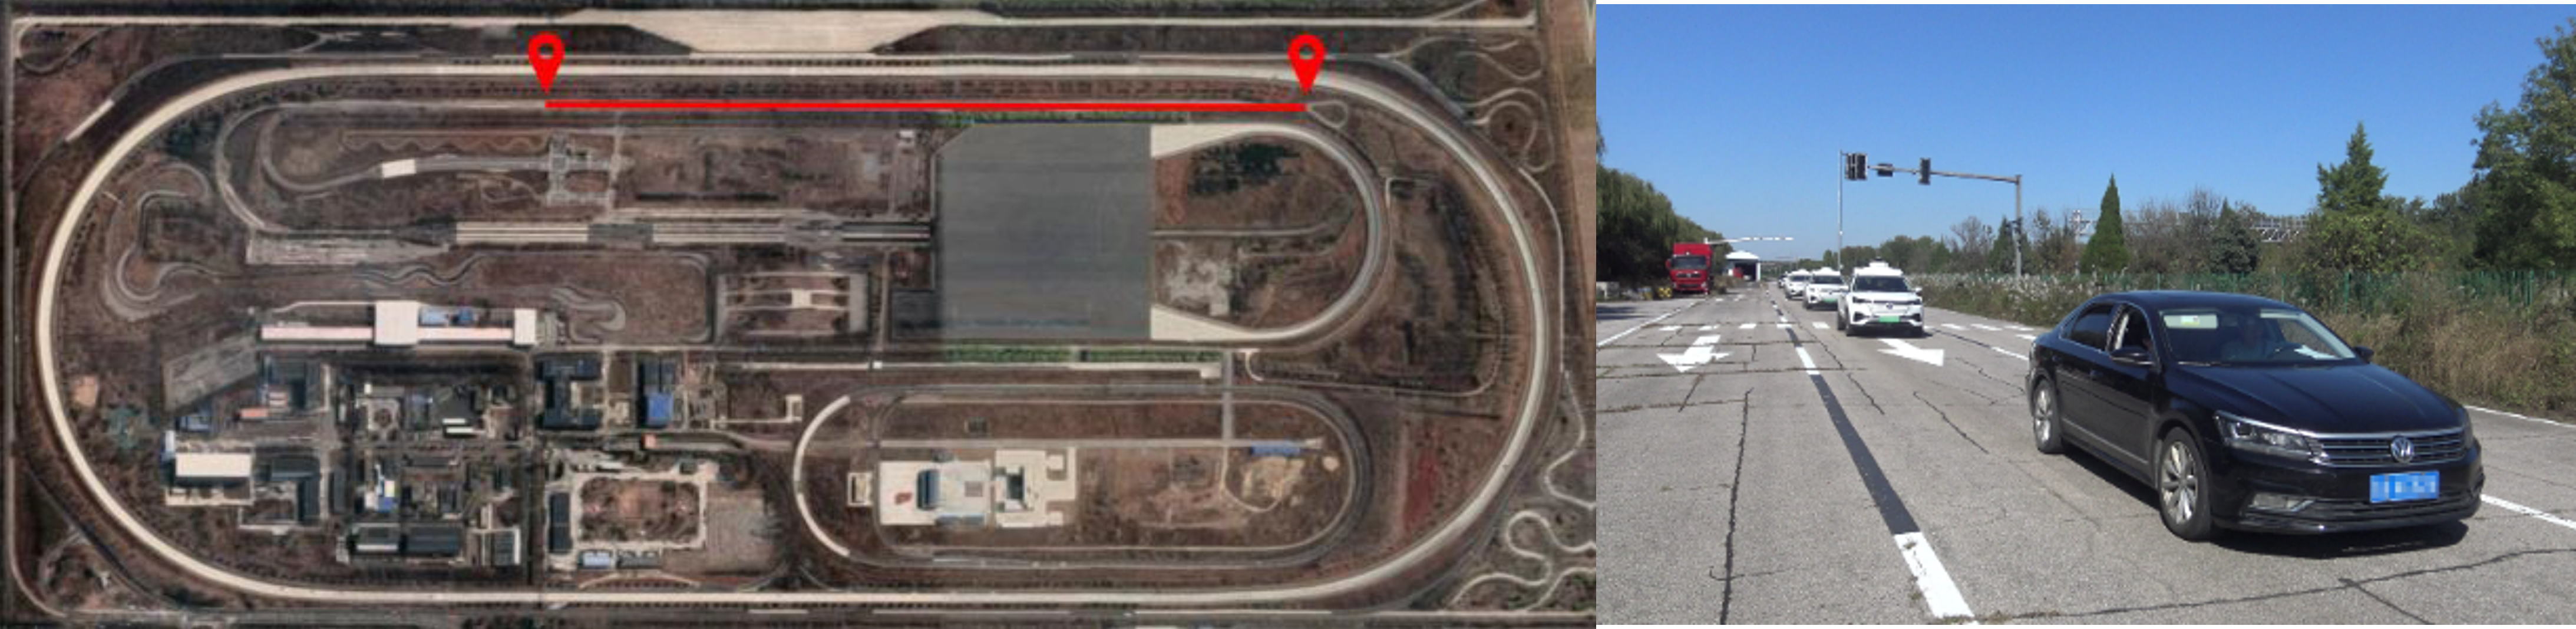
\includegraphics[width=0.55\textwidth]{figs/fig2.png}
  \caption
  {~The adopted representative leader maneuvers: (a) and (b) denote the velocity and acceleration signal of the NGSIM field data, respectively.} 
  \label{fig2}
\end{figure}

A platoon of five vehicles, consisting of one exogenous leader and four controlled followers connected by MPLF topology, is set up for the numerical simulations. The leader CACC's acceleration and speed profiles are adopted from the Next Generation Simulation (NGSIM) field data, a representative leader maneuver \citep{montanino2013making}, as illustrated in Fig.~\ref{fig2}. It should be noted that the above profiles are applied to the leader CACC once the platoon reaches an equilibrium state in which all CACCs move at the same speed while maintaining the desired time headway. Additionally, the simulation parameters are presented in Table\ref{table1}.

\begin{table}
  \centering
  \setlength{\abovecaptionskip}{0pt}
  \setlength{\belowcaptionskip}{10pt}%设置标题与表格的距离
  \begin{threeparttable}[b]
    \caption{~Overview of the parameters for the simulations.}
    \label{table1}
    {\begin{tabular}{lc} \toprule
        Parameters                              & Value                \\ \midrule
        Platoon size $n$                        & 5 vehicles           \\
        Vehicle length $L$                      & 5 [m]                \\
        Engine actuator delay $\tau_i$                     & 0.2 [s] \tnote{1}   \\
        Upper bound of the rate-free communication delay $h$ & 0.4 [s]              \\
        Weight of communication link (i,j) $a_{ij}$                 &  $\frac{1}{d_i}$ \\
        Desired time headway [s] & $0.6s$\\
        Control parameters & $k_i=[0.3,0.3,0.3]^T$ \\
        \bottomrule
      \end{tabular}}
    \begin{tablenotes}
      \item[1] \citep{Wang2018a,Zhou2020}
    \end{tablenotes}
  \end{threeparttable}
\end{table}



To investigate the effects of a rate-free communication delay and measurement uncertainties on tracking performance, transient response, and safety conditions, specific analyses are conducted on the following three cases:
\begin{enumerate}
  \item \textit{Case \uppercase\expandafter{\romannumeral1}} Deterministic system: A deterministic system is assumed, where the communication delay is set to a constant value, such as the upper bound of the rate-free communication delay $h$, and system uncertainties are not taken into account.
  \item \textit{Case \uppercase\expandafter{\romannumeral2}} Rate-free communication delay: The communication delay is set to be rate-free and follows a Poisson random distribution with a mean of $0.2s$ and an upper bound of $0.4s$ \citep{ko1984delay,geng2008millimeter,consul1973generalization}. Similarly, system uncertainties are not considered.
  \item \textit{Case \uppercase\expandafter{\romannumeral3}} Uncertain system: An uncertain system is considered, where both the rate-free communication delay and system uncertainties are taken into account. The rate-free communication delay is set the same as in Case \uppercase\expandafter{\romannumeral2}. Dynamic system uncertainties are presumed to solely influence the measurement process of the vehicle system, and they are defined accordingly:
  \begin{equation*}
 D=I, 
  \end{equation*}
  \begin{equation*}
    F(t)=\sin t, 
     \end{equation*}
     \begin{equation*}
      E=I_n \otimes\left[\begin{array}{ccc}
        0 & 0.05 & 0 \\
        0 & 0 & 0.05 \\
        0 & 0 & 0.05
        \end{array}\right], 
       \end{equation*}
       \begin{equation*}
        E_{d}=R \otimes\left[\begin{array}{ccc}
          0 & 0 & 0 \\
          0 & 0 & 0 \\
          0.1 & 0.1 & 0.1
          \end{array}\right] ,
         \end{equation*}
         \begin{equation*}
          R=\left[\begin{array}{lllll}
            0 & 0 & 0 & 0 & 0 \\
            1 & 0 & 0 & 0 & 0 \\
            0 & 1 & 0 & 0 & 0 \\
            0 & 0 & 1 & 0 & 0 \\
            0 & 0 & 0 & 1 & 0
            \end{array}\right].
           \end{equation*}
  
        % \begin{equation*}
        %   \left\{ \begin{aligned}
        %     & D=I, \\
        %     & F(t)=\sin t ,\\
        %     & E=I_n \otimes\left[\begin{array}{ccc}
        %     0 & 0.05 & 0 \\
        %     0 & 0 & 0.05 \\
        %     0 & 0 & 0.05
        %     \end{array}\right], \\
        %     & E_{d}=R \otimes\left[\begin{array}{ccc}
        %     0 & 0 & 0 \\
        %     0 & 0 & 0 \\
        %     0.1 & 0.1 & 0.1
        %     \end{array}\right] \text {, } \\
        %     & R=\left[\begin{array}{lllll}
        %     0 & 0 & 0 & 0 & 0 \\
        %     1 & 0 & 0 & 0 & 0 \\
        %     0 & 1 & 0 & 0 & 0 \\
        %     0 & 0 & 1 & 0 & 0 \\
        %     0 & 0 & 0 & 1 & 0
        %     \end{array}\right]. \\
        %     \end{aligned}
        %   \right.
        % \end{equation*}
\end{enumerate}

% possion distribution加参考文献。
Furthermore, corresponding matrices $M$, $N$, $Y$, $L_1$, and $L_2$, with a scalar $\varepsilon$ that satisfy Theorems~\ref{theorem6} and~\ref{theorem7}, can be found in Appendix C. An in-depth analysis is conducted on the tracking performance, transient response, and safety conditions.



\subsection{Tracking performance analyses}
\label{Section 5.2}

Upon the formation of all CACCs into a CACC platoon and attainment of the equilibrium state, the leader maneuver, depicted in Fig.\ref{fig2} from NGSIM, is executed by the Leader CACC. The tracking performance results for the three cases are showcased in Fig.\ref{fig3}. It is important to highlight that in \textit{Cases \uppercase\expandafter{\romannumeral2} and \uppercase\expandafter{\romannumeral3}}, the communication delay is rate-free. Consequently, the tracking error, encompassing spacing and velocity errors, is derived from the actual trajectory rather than the error employed in the decision-making process.






\begin{figure}
  \centering
  \includegraphics[width=\textwidth]{figs/fig3.png}
  \caption
  {~Tracking performance of the CACC platoon under the NGSIM field data for the three \textit{Cases}: (a), (b), (c), and (d) present tracking results under \textit{Cases \uppercase\expandafter{\romannumeral1}}, including the velocity, acceleration, tracking error of spacing, and tracking error of velocity, respectively; (e), (f), (g), and (h) show the case under \textit{Cases \uppercase\expandafter{\romannumeral2}}; (i), (j), (k), and (l) denote the case under \textit{Cases \uppercase\expandafter{\romannumeral3}}.} 
  \label{fig3}
\end{figure}

As anticipated from theoretical findings, all the CACCs exhibit the ability to smoothly track the leader maneuver with a steady-state error of 0. Transient fluctuations in the leader maneuver are observed to generate variations in the followers' tracking error, which progressively diminish over time as stability is maintained. Additionally, although not overtly apparent in the velocity and acceleration subplots, the introduction of the rate-free communication delay and measurement uncertainties is found to augment the tracking error, consequently impairing tracking performance under equivalent leader maneuvers.






\subsection{Transient response analyses}
\label{Section 5.3}

In Section~\ref{Section 5.2}, the analysis pertaining to tracking performance delivers qualitative results. To conduct a quantitative analysis, it is essential to utilize two widely acknowledged metrics for assessing transient response: Settling Time (ST) and Maximum Overshoot (MO). The ST is defined as "the time required for the response curve to reach and stay within a range of a certain percentage (5\%) of the final value," while the MO is described as "the maximum peak value of the response curve measured from the desired response of the system" \citep{ogata1995discrete}. Among these two metrics, the ST denotes the duration required for the controller to transition from the transient response to a steady-state, symbolizing speed, whereas the MO signifies the peak deviation of the controller's excited transient response from the steady state, representing accuracy. According to their definitions, smaller ST and MO values are associated with superior transient response, enhanced driving comfort, and increased safety \citep{na2017active}.

\begin{figure}
  \centering
  \includegraphics[width=\textwidth]{figs/fig4.png}
  \caption
  {~Metrics for evaluating the transient response of each CACC among the CACC platoon under the three \textit{Cases}: (a) the case of setting time; (b) the case of maximum overshoot.} 
  \label{fig4}
\end{figure}

Figure~\ref{fig4} exhibits the outcomes of the two metrics for three distinct cases, where CACC2, CACC3, CACC4, and CACC5 refer to the second, third, fourth, and fifth CACC in the CACC platoon, respectively. In accordance with the qualitative analysis, the incorporation of the rate-free communication delay and measurement uncertainties indeed exacerbates the transient response. To elaborate, for CACC5, introduction of the rate-free communication delay leads to a 401.9\% increase in ST and an 88.7\% increase in MO, while the introduction of measurement uncertainties results in a 9.2\% increase in ST and a 16.4\% increase in MO. Moreover, both the ST and MO values decline as the vehicle index escalates, signifying that vehicles positioned further back in the platoon attain a steady state more rapidly and precisely. This enhancement can be attributed to the capacity of vehicles situated further back in the platoon to access more distant and diverse information, thereby facilitating control decision-making.




\subsection{Safety condition analyses}
\label{Section 5.4}


To evaluate the effect of the rate-free communication delay and measurement uncertainties on safety, another quantitative analysis is conducted based on an additional safety metric, Deceleration Rate to Avoid a Crash (DRAC) \citep{meng2011evaluation}. DRAC is a widely accepted metric for assessing safety and is defined as the minimum required deceleration rate that a vehicle must apply to avoid a collision with the leading vehicle. The DRAC can be formulated for each vehicle $i$ at time $t$ as follows:
\begin{equation*}
  DRAC{_i}(t) = \frac{{{{\left( {{v_i}(t) - {v_{i - 1}}(t)} \right)}^2}}}{{2\left( {{p_{i - 1}}(t) - {p_i}(t) - L} \right)}}
\end{equation*}

\begin{figure}
  \centering
  \includegraphics[width=0.65\textwidth]{figs/fig5.png}
  \caption
  {~The boxplots of DRAC for the entire simulation period of each \textit{Case} under investigation: (a) \textit{Cases \uppercase\expandafter{\romannumeral1}}; (b) \textit{Cases \uppercase\expandafter{\romannumeral2}}; (c) \textit{Cases \uppercase\expandafter{\romannumeral3}}.} 
  \label{fig5}
\end{figure}

\begin{table}
  \centering
  \setlength{\abovecaptionskip}{0pt}
  \setlength{\belowcaptionskip}{10pt}%设置标题与表格的距离
    \caption{~Descriptive statistics of DRAC for the entire simulation period of different Cases.}
    \label{table2}
    {\begin{tabular}{lccc} \toprule
        Case index                              & 
         Mean       & Median    &  Range    \\ \midrule
        \textit{Case \uppercase\expandafter{\romannumeral1}}                   & 0.01426  & 0.00096 &  1.23604     \\
        \textit{Case \uppercase\expandafter{\romannumeral2}}      & 0.01567 & 0.00116 &   1.35961         \\
        \textit{Case \uppercase\expandafter{\romannumeral3}}                    & 0.01469 & 0.00101 &  1.49666 \\
        \bottomrule
      \end{tabular}}
\end{table}

Figure~\ref{fig5} presents the DRAC for the entire simulation period in the form of boxplots. It is evident that the introduction of the rate-free communication delay increases DRAC, making collision-prone scenarios more probable. Consequently, real-world scenarios with the rate-free communication delay exhibit worse safety conditions compared to ideal scenarios with constant communication delay, which aligns with the conclusions drawn from transient response analyses in Section~\ref{Section 5.3}. Simultaneously, a counterintuitive conclusion is deduced based on smaller DSRC values that measurement uncertainties appear to benefit safety conditions. We speculate that this observation may arise from the fact that boxplots focus on data within 1.5 times the interquartile range, considering other data points as outliers. Therefore, descriptive statistics of all DRAC for different cases are provided in Table.~\ref{table2} for further quantitative analysis. It can be observed that although uncertainties reduce DRAC most of the time, they increase the range, which indicates that scenarios with adverse safety conditions are more likely to occur. Furthermore, DRAC significantly decreases as the vehicle index increases, suggesting that CACCs with more distant and diverse information have better safety conditions.







\section{Conclusion and future work}
\label{Section 6}

This paper presents a general representation for a CACC platoon considering a rate-free communication delay based on graph theory and supermatrix. A novel stability condition is derived based on the Lyapunov-Krasovskii Stability Theorem and Schur complement to overcome the rate-free attribute of communication delays. Furthermore, another robust stability condition is also deduced, considering the presence of measurement uncertainties. Extensive numerical analyses are conducted to investigate the impact of a rate-free communication delay and measurement uncertainties on tracking performance, transient response, and safety conditions. The following conclusions can be drawn through numerical analysis:
\begin{enumerate}
  \item By employing the Lyapunov-Krasovskii Stability Theorem and Schur complement, a stability condition for a CACC platoon that accounts for a rate-free communication delay can be derived.
  \item In all cases, if the stability condition is fulfilled, all CACCs can effectively track errors and achieve equilibrium.
  \item Realistic scenarios with a rate-free communication delay and measurement uncertainties exhibit poorer tracking performance, transient response, and safety conditions compared to ideal scenarios featuring constant communication delay.
  \item CACCs with access to more distant and diverse information demonstrate superior transient response and safety conditions.
\end{enumerate}
Nevertheless, we recognize that the vehicle behavior in the simulation merely represents a simplified version of reality, and additional field experiments are required to deliver a more precise analysis of the tracking performance. Furthermore, the vehicle dynamics employed in this paper are linearized, while in reality, they are nonlinear, which poses challenges for stability analysis. Moreover, future research should also focus on developing innovative control strategies to facilitate smoother and safer tracking performance.



\appendix


\section*{Appendix A.~Feedback control for linearization}
\label{AppendixA}
In this appendix, we present the linearization of the longitudinal vehicle dynamics described in Equation (\ref{eq3}). The uncertain resistance forces, which include $f_i^g(t)$, $f_i^w(t)$, and $f_i^r(t)$, can be expressed as follows:
\begin{equation}
  \left\{\begin{array}{l}
    f_{i}^{g}(t)=m_{i} g \sin \left(\theta_{i}(t)\right),                        \\
    f_{i}^{w}(t)=\frac{1}{2} \rho C_{D} A_{F}\left(v_{i}(t)+v_{w}(t)\right)^{2}, \\
    f_{i}^{r}(t)=\mu_{R} m_{i} g \cos \left(\theta_{i}(t)\right).
  \end{array}\right.
  \label{eqapp5}
\end{equation}
where $g$ is the acceleration of gravity; $\theta_i(t)$ denotes the inclination angle of the road; $\rho$ represents the air density; $C_D$ is the coefficient of aerodynamic drag; $A_F$ denotes the maximal cross-sectional/frontal area of the vehicle; $v_w(t)$ represents the uncertain headwind speed; and $\mu_R$ is the coefficient of rolling resistance.


The desired engine dynamic is modeled as follows:
\begin{equation}
  (\tau_is+1)F_i^e=U_i.
  \label{eqapp6}
\end{equation}

Applying the inverse Laplace transformation to Equation (\ref{eqapp6}) yields:
\begin{equation}
  \dot{f_i^e}\left(t\right)=\frac{u_i(t)}{\tau_i}-\frac{f_i^e\left(t\right)}{\tau_i}.
  \label{eqapp7}
\end{equation}

Upon substitution of Equation (\ref{eq3}) into Equation (\ref{eqapp7}), and differentiation of both sides with respect to time, the resulting equation is:
\begin{small}
\begin{equation}
  \begin{aligned}
    \dot{a}_{l}(t) & =\frac{\dot{f}_{l}^{e}(t)}{m_{i}}-\frac{\dot{f}_{l}^{g}(t)}{m_{i}}-\frac{f_{l}^{i \omega}(t)}{m_{i}}-\frac{\dot{f}_{l}^{r}(t)}{m_{i}}                                                                                         \\
                   & =               \frac{u_{i}(t)}{m_{i} \tau_{i}}                                                                                                                                                                               \\
                   & -               \frac{a_{i}(t)+\mathrm{g} \sin \left(\theta_{i}(t)\right)\left[1-\tau_{i} \mu_{R} \dot{\theta}_{l}(t)\right]+\mathrm{g} \cos \left(\theta_{i}(t)\right)\left[1+\tau_{i} \dot{\theta}_{l}(t)\right]}{\tau_{i}} \\
                   & -               \frac{\frac{1}{2} \rho C_{D} A_{F}\left(v_{i}(t)+v_{w}(t)\right)\left(\left(v_{i}(t)+v_{w}(t)\right)+2 \tau_{i}\left(a_{i}(t)+\dot{v}_{w}(t)\right)\right)}{\tau_{i}}.
  \end{aligned}
  \label{eqapp8}
\end{equation}
\end{small}

Therefore, the nonlinear state feedback utilized for linearization can be defined as:
\begin{equation}
  \begin{aligned}
    u_i^\ast\left(t\right)= & m_iu_i\left(t\right)+g\sin{\left(\theta_i\left(t\right)\right)}\left[1-\tau_i\mu_R\dot{\theta_i}\left(t\right)\right]\\
    &+g\cos{\left(\theta_i\left(t\right)\right)}\left[1+\tau_i\dot{\theta_i}\left(t\right)\right]\ \\
                            & +\frac{1}{2}\rho C_DA_F\left(v_i\left(t\right)+v_w\left(t\right)\right)\\
                            &\quad \left(\left(v_i\left(t\right)+v_w\left(t\right)\right)+2\tau_i(a_i\left(t\right)+\dot{v_w}\left(t\right))\right).
  \end{aligned}
  \label{eqapp9}
\end{equation}

The Equation (\ref{eq3}) can be reformulated under the new feedback control input as follows:
\begin{equation}
  \tau_i\dot{a_i}\left(t\right)+a_i\left(t\right)=u_i(t).
  \label{eqapp10}
\end{equation}


\section*{Appendix B.~Connection between Lyapunov-Krasovskii Stability Theorem and second Lyapunov method.}
\label{AppendixCCC}

We begin by stating a lemma related to the Lyapunov function:
\begin{lemma}
  \label{lemmaYY}
  \citep{Kolmanovskii1999}. Consider a system $\dot{X}(t)=f(X(t), X(t-\phi\left(t\right)))$ with $f\left(0,0 \right)= 0$. Assume the existence of a Lyapunov function $F:G\rightarrow\mathbb{R}$, where $X,y\in G$ and $F\left(y\right)<F\left(X\right)$ implies that:
  \begin{equation}
    \left(\dot{F}\left(X\right)f\left(X,y\right)\right)\left(\ddot{F}\left(X\right)f\left(X,y\right)\right)\le0.
  \end{equation}

  Then the solution $X(t)\equiv0$ is stable.
\end{lemma}

The functional $V:\mathcal{C}\rightarrow\mathbb{R}$ is defined as follows, given the existence of a Lyapunov function $F:\mathbb{R}^n\rightarrow\mathbb{R}$:
\begin{equation}
  V(\Phi ): = \mathop {\max }\limits_{ - h \le \theta  \le 0} F(\Phi (\theta )),(\forall \Phi  \in \mathcal{C}).
  \label{yy1}
\end{equation}

By definition, the following conditions hold:
\begin{small}
\begin{equation}
  \dot{V}(\Phi)\left\{\begin{array}{cl}
    \leq 0,                                                          & \text { if } F(\Phi(0))<V(\Phi), \\
    =\max \left(\dot{F}(\Phi(0)), f(\Phi(0), \Phi(-\phi(t))), 0\right), & \text { if } F(\Phi(0))=V(\Phi),
  \end{array}\right.
\end{equation}
\end{small}
where $f(\Phi(0), \Phi(-\phi(t)))=\Psi\Phi(0)+\Psi_d\Phi(-\phi(t))$.

The condition in which $\dot{V}\left(\Phi\right)>0$ holds is dependent on the following:
\begin{equation}
  F(\Phi (0)) = \mathop {\max }\limits_{ - h \le \theta  \le 0} F(\Phi (\theta ))\;and(\dot F(\Phi (0)),f(\Phi(0), \Phi(-\phi(t)))) > 0.
  \label{yy3}
\end{equation}

In a neighborhood $G\subset\mathbb{R}^n$, the function $F$ can be defined. Subsequently, the functional $V$ can be defined for $\Phi\in\mathcal{C}$ with values in $G$.


If Equation~(\ref{yy3}) holds for some functions $\Phi\in\mathcal{C}$, then the inequality $F\left(\Phi\left(-\phi\left(t\right)\right)\right)<F\left(\Phi\left(0\right)\right)$ can be obtained, which makes $\Phi$ arbitrarily small. This implies that the second condition in Equation~(\ref{yy3}) still holds, but it conflicts with Lemma~\ref{lemmaYY}. Therefore, it can be concluded that $\dot{V}\left(\Phi\right)\le0$ holds constantly for all $\Phi$.


Therefore, the Lyapunov-Krasovskii Stability Theorem can be regarded as an extension of the second Lyapunov method to functional space. Unlike the second Lyapunov method, this extension does not introduce any additional constraints since it only requires definite sign at the start and end points instead of in the entire neighborhood. Therefore, stability conditions obtained using the Lyapunov-Krasovskii Stability Theorem are more accurate than those obtained using the second Lyapunov method. This conclusion has been supported by previous research \citep{wang2016fuzzy,lian2020dissipativity}.





\section*{Appendix C.~Attachments uploaded to GitHub}
\label{AppendixB}
The code uploaded for this paper includes the formulation of Theorem~\ref{theorem4} and the construction of LMIs for Theorems~\ref{theorem6} and \ref{theorem7}. Matrices corresponding to the three cases in Section~\ref{Section 5}, which are compatible with Theorem~\ref{theorem7}, have also been included in the repository. The URL for the file repository is:\\ 
https://github.com/ruantiancheng/code-paper-82.

\printcredits

\section*{Acknowledgment}

This research was sponsored by the National Key Research and Development Program of China (No. 2022ZD0115600), and National Science Foundation of China (No. 52072067), and Postgraduate Research \& Practice Innovation Program of Jiangsu Province (KYCX22\_0266).

%% Loading bibliography style file
% \bibliographystyle{model1-num-names}
\bibliographystyle{cas-model2-names}

% Loading bibliography database
\bibliography{cas-refs}


%\vskip3pt

\end{document}

